\subsection{Pseudo Random Number Generators}
When producing a synthetic dataset, there is a need for a lot of random numbers. Many programming languages have a built-in function that produces numbers that appear random, but actually are not. Computers are deterministic machines, and therefore cannot produce a number without some sort of algorithm. If the algorithm is known, it becomes possible to predict the next number; hence the numbers are not completely random. Random numbers should be independent; that is, each number should have no connection to any previously produced values. The distribution should also be uniform, meaning if you generate 1,000,000 random numbers in the range [0,1), you'd expect about 500,000 values in [0, 0.5) and about 500,000 in [0.5, 1). Earlier in history, these numbers have been produced by flipping coins or rolling dice. Today, it is possible to produce truly random numbers by using atmospheric noise. Despite its potential advantages, this method requires significant resources, making it inefficient for the intended application. Therefore, pseudo-random numbers will be used instead.
\newline

\noindent Pseudo-random numbers behave like random numbers but are deterministically generated from a seed value. While
these numbers are not truly random, they are sufficiently unpredictable for many practical applications.
To generate the data, we use a Pseudo-Random Number Generator, also known as a PRNG.
PRNGs are algorithms that produce sequences of numbers that appear random.
\newline

\noindent Random numbers are widely used in fields such as statistics, game theory, cryptography, and simulations. These applications require numbers that behave
as if they were random, yet can be reproduced when needed. This is where
PRNGs come in. They allow for repeatable randomness, making them ideal for
controlled experiments, testing, and security.
\\
This chapter will explore the key concepts behind PRNGs. Before going into the
mechanics of these generators, it is important to first understand what ’random’
means and the characteristics that define truly random numbers.

\subsubsection{Properties of PRNGs}

The quality of a PRNG is determined by several key factors that influence its
use for different applications. Some of the properties of a good PRNG are independence, a long period and reproducibility
\newline \\
The numbers produced by the PRNG should be statistically independent, en-
suring that each generated value exhibits no correlation with previous numbers
or other sequences. This implies that knowledge of previously generated num-
bers or sequences provides no advantage in predicting the next output.
\newline \\
A PRNG operates within a specific interval before its sequence begins to repeat.
A high-quality PRNG has a long interval, delaying repetition and enhancing its
unpredictability. Conversely, a PRNG with a shorter period becomes more pre-
dictable and less suitable for practical use.
\newline \\
A key feature of a PRNG is its ability to reproduce the same sequence of num-
bers when given a specific seed. This property is particularly useful in testing
and simulation scenarios, where it is essential to generate identical sequences
multiple times for consistency and reproducibility.
\newline \\
In addition, a PRNG must be fast and efficient to prevent it from introducing
performance bottlenecks within an application. The speed of number generation
directly impacts computational efficiency, especially in applications requiring a
large volume of random numbers. An inefficient PRNG can significantly slow
down processes, undermining the overall performance of the system. Therefore,
balancing randomness and efficiency is essential for practical applications

\subsubsection{Linear Congruential Generator}

Linear Congruential Generator (LCG) is a commonly used approach to generate
pseudo-random numbers. LCG generates a sequence of numbers using a linear
recurrence relation, expressed as:

\begin{equation}
X_{n+1} = (aX_n + c) \bmod m \cite{knuth}.
\end{equation}

\noindent $X_0$ is the seed value and must be in the range $0 \leq X_0 < m$ \newline
$a$ is the multiplier,\newline 
$c$ is the increment and \newline
$m$ is the modulus, which specifies the range of values. $m$ must be greater than 0 \newline
\\
\noindent The operation 'mod $m$' represents division by $m$, where only the remainder
is retained. This ensures that the generated number remains within the range
0 to $m-1$.  $X_0$, $a$ and $c$ must all be in the interval $[0, m)$. 
Here is an example of the first 4 numbers of a sequence given these parameters: \newline

\begin{equation}
	a = 5, c = 1, m = 16, and X_0 = 7:
\end{equation}

\begin{equation}
	 X_1 = (5 \cdot 7 + 1)\bmod 16 = 4.
\end{equation}
\begin{equation} 
	X_2 = (5 \cdot 4 + 1) \bmod 16 = 5. 
\end{equation}
\begin{equation} X_3 = (5 \cdot 5 + 1) \bmod 16 = 10. \end{equation}
\begin{equation} X_4 = (5 \cdot 10 + 1) \bmod 16 = 3. \end{equation}
\\
\noindent This sequence has a period of 16. In an LCG, the period can be as large as $m$,
because the remainder after division by $m$ will always be less than or equal to
$m$. Consequently, choosing a large $m$ is typically desirable, as it can potentially
lead to longer periods. However, the period length is not determined solely by
$m$; the choice of other parameters—such as the multiplier, increment, and the
seed, along with their relationships, significantly impact the overall period. It
is possible to select a larger $m$ and still end up with a shorter period if the parameters are not chosen properly. Here is an example where a larger $m$ results in a shorter period, illustrating that.

\begin{center}
	$a=4$, $c=6$, $m=20$, $X_0=3.$
\end{center}

\begin{equation} X_1=(4 \cdot 3 +6)=18 \bmod 20=18.\end{equation}
\begin{equation}X_2=(4 \cdot 18+6)=78 \bmod 20=78 \bmod 20=18.\end{equation}

\noindent Here a larger $m$ is used, but a shorter period of 1 appears. 
\newline \\
The selection of the optimal parameters for a LCG would be excessive for the objective of this project, it is beyond the scope of this project and will therefore not be addressed further.

\subsubsection{Test of PRNG}
As stated previously, the length of the sequence produced by the PRNG is not the only important factor. A uniform distribution and independence of each generated number is significant too. If these criteria are not met, there will be correlation between the generated numbers, which means that the randomness is of low quality. For example, consider a sequence that follows the three-times-table, with the first number being 3: (3,6,9,12,...). In that sequence, it is pretty easy to guess the upcoming number, based on the previous one. Normally the correlations are harder to spot than this example, which is why it is important to test the quality of a PRNG.
\newline

\noindent There are different tests used to evaluate PRNG quality and performance, including the Kolmogorov-Smirnov test, chi-squared test and the spectral test \cite{knuth}. Passing one of these tests does not mean that it will pass others. Therefore, every test that it passes, just makes it more likely to produce a high quality sequence. One of the important tests for LCG is the spectral test. Another advantage of the spectral test in the context of this paper is that it can be visualized in two or three dimensions, which can make it easier to understand.
\newline

\noindent The test looks at how the numbers in the sequence are distributed in different dimensions. If hyperplanes and lines occur, as seen on Figure \ref{fig:badspec2d} and Figure \ref{fig:badspec3d}, generated by $X_{n+1}=137\cdot X_{n}+187$ mod $256$, the sequence fails the test, since the distribution is not random.
\newline

\noindent Looking at the spectral test used on a LCG with the parameters from the Park-Miller Minimal Standard\:  $X_{n+1}=(48271\cdot X_{n}) \text{ mod } (2^{31}-1)$\cite{knuth}, on Figure \ref{fig:goodspec2d} and Figure \ref{fig:goodspec3d}, the hyperplanes will not always be visible in 2d or 3d, but only in higher dimensions. Therefore a visual examination will not be enough to conclude the complete quality of a PRNG. Methods for inspecting LCGs in these dimensions do exist, but will not be mentioned in this project
\newline

\noindent In this project, the PRNG used will be the Mersenne-Twister. It has very good properties, uniformity and a period of $2^{19937}-1$ and passes the spectral test \cite{mersenne}. The test in 2D and 3D can be seen on figure \ref{fig:msspec2d} and figure \ref{fig:msspec3d}. Another reason for this choice is that Mersenne-Twister is the built-in generator in R, which makes it convenient. 


%Spectral test for bad LCG
\begin{figure}
	\centering
	\begin{minipage}{0.45\textwidth}
		\centering
		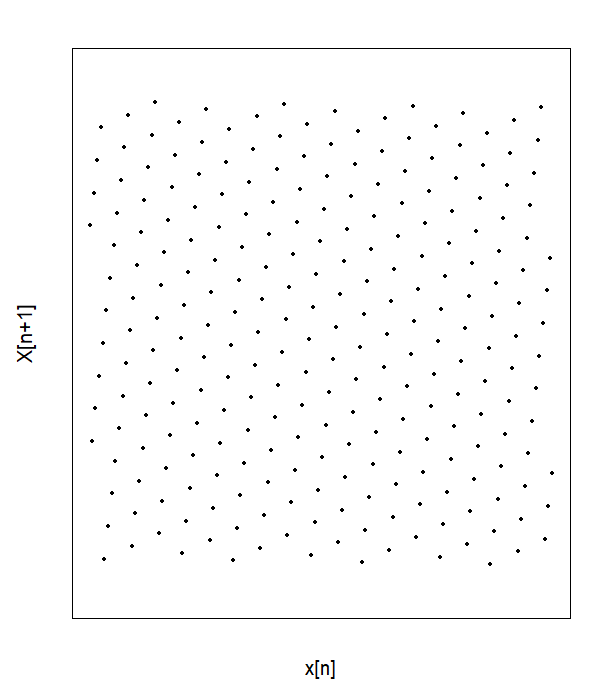
\includegraphics[width=\linewidth]{billder/spec_bad_lcg_2d.png}
		\caption{2D spectral test for LCG using bad parameters: $X_{n+1}=(137\cdot X_{n}+187) \text{ mod } 256$.}
		\label{fig:badspec2d}
	\end{minipage}\hfill
	\begin{minipage}{0.45\textwidth}
		\centering
		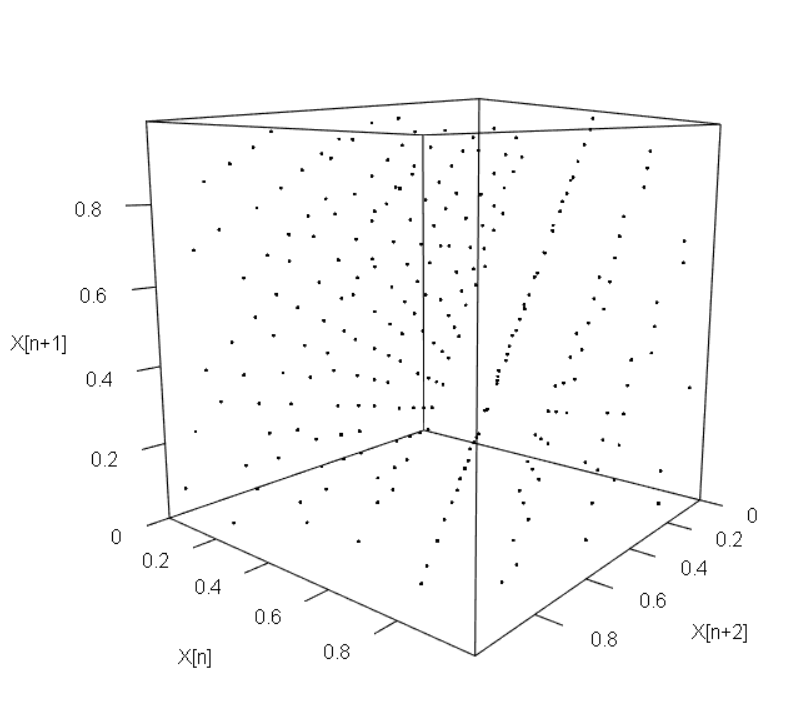
\includegraphics[width=\linewidth]{billder/spec_bad_lcg_3d.png}
		\caption{3D spectral test for LCG using bad parameters: $X_{n+1}=(137\cdot X_{n}+187) \text{ mod } 256$.}
		\label{fig:badspec3d}
	\end{minipage}
\end{figure}

%Spectral test good LCG
\begin{figure}
	\centering
	\begin{minipage}{0.45\textwidth}
		\centering
		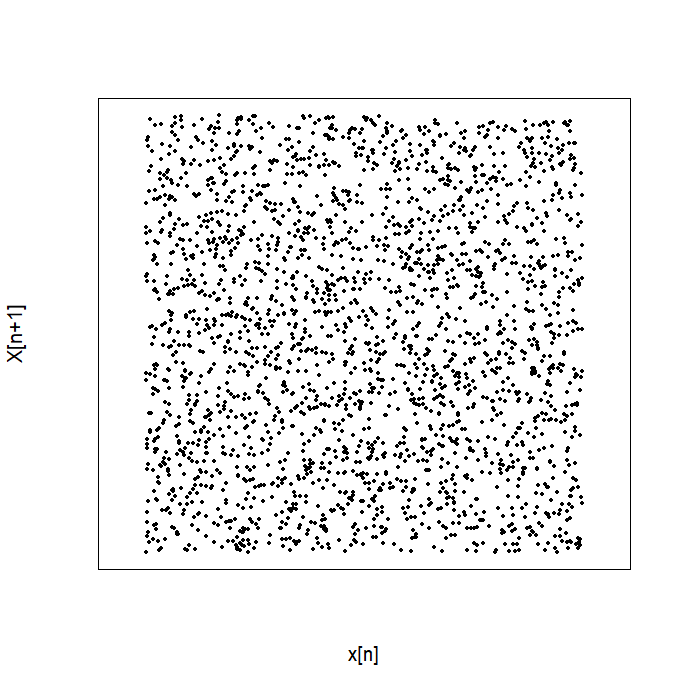
\includegraphics[width=\linewidth]{billder/spec_good_lcg_2d.png}
		\caption{2D spectral test for LCG using good parameters: $X_{n+1}=(48271\cdot X_{n}) \text{ mod } (2^{31}-1)$.}
		\label{fig:goodspec2d}
	\end{minipage}\hfill
	\begin{minipage}{0.45\textwidth}
		\centering
		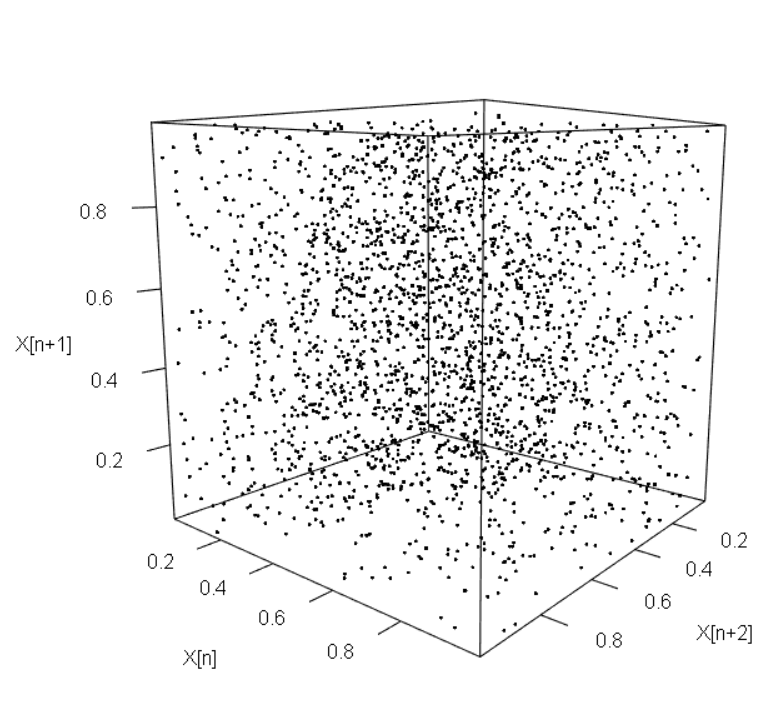
\includegraphics[width=\linewidth]{billder/spec_good_lcg_3d.png}
		\caption{3D spectral test for LCG using good parameters: $X_{n+1}=(48271\cdot X_{n}) \text{ mod } (2^{31}-1)$.}
		\label{fig:goodspec3d}
	\end{minipage}
\end{figure}

%Mersenne-Twister spectral tests
\begin{figure}
	\centering
	\begin{minipage}{0.45\textwidth}
		\centering
		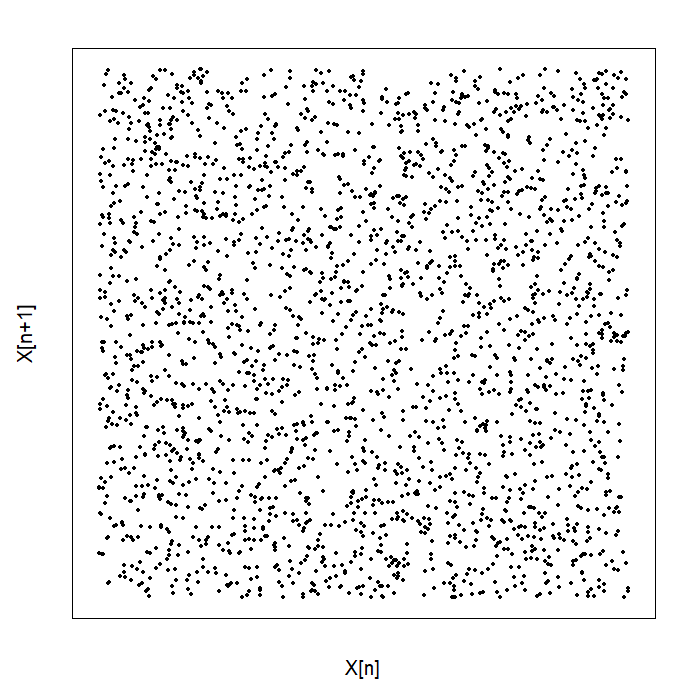
\includegraphics[width=\linewidth]{billder/ms_spec_2d.png}
		\caption{2D Spectral test for the PRNG Mersenne-Twister, in R.}
		\label{fig:msspec2d}
	\end{minipage}\hfill
	\begin{minipage}{0.45\textwidth}
		\centering
		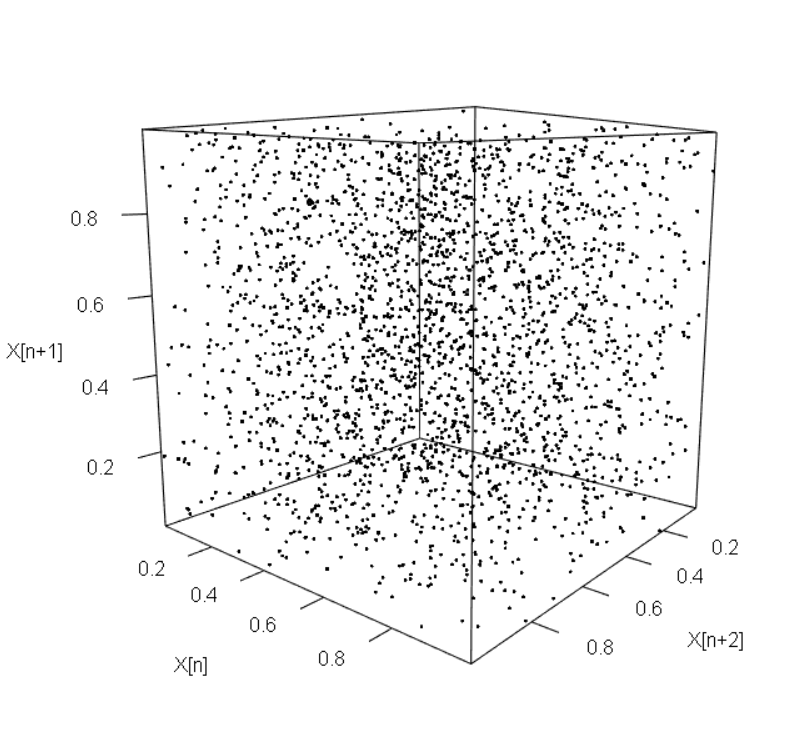
\includegraphics[width=\linewidth]{billder/ms_spec_3d.png}
		\caption{3D Spectral test for the PRNG Mersenne-Twister, in R.}
		\label{fig:msspec3d}
	\end{minipage}
\end{figure}

\newpage
